% Front and back cover pages for the white-paper book (kultem colours).
% Front image: 3.5ST_in_space.png   Back image: 3.5ST_in_KASI.png

\newcommand{\MakeFrontCover}{%
  \begin{titlepage}
  \thispagestyle{empty}\sffamily\centering
  % --- title banner ---
  \noindent\colorbox{Blue3}{\parbox[t]{\dimexpr\textwidth-2\fboxsep\relax}{%
    \vspace{4mm}\centering
    {\color{white}\bfseries\fontsize{24}{29}\selectfont 3.5-meter Segmented-Mirror\\[1.5mm]
      Robotic Space Telescope}\\[3.5mm]
    {\color{white}\Large Mission White Paper}\\[1.5mm]
    {\color{white!88}\large Overall Architecture and Scientific Mission}%
    \vspace{4mm}}}
  \vfill
  % --- cover image ---
  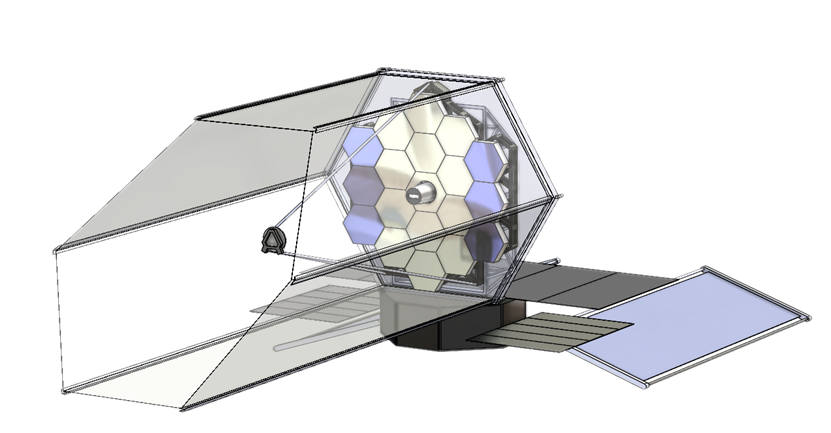
\includegraphics[width=\textwidth]{3.5ST_in_space.png}
  \vfill
  % --- authors and affiliations ---
  {\color{ink}\bfseries\normalsize \wpauthors\par}
  \vspace{3mm}
  {\color{muted}\small Korea Astronomy and Space Science Institute \textperiodcentered\
    Space Telescope Science Institute\\
    Korea Institute for Advanced Study \textperiodcentered\ Pusan National University \\ Korea National University of Education\textperiodcentered\
    Seoul National University\par}
  \vspace{5mm}
  {\color{Blue3}\bfseries\Large 2026}
  \vspace{4mm}
  \end{titlepage}}

% Inside front cover: copyright / distribution notice / citation (colophon).
\newcommand{\MakeColophon}{%
  \clearpage
  \thispagestyle{empty}\sffamily
  \null\vfill
  \noindent{\color{muted}\footnotesize
    {\color{ink}\bfseries 3.5-meter Segmented-Mirror Robotic Space Telescope}\\
    Mission White Paper: Overall Architecture and Scientific Mission\\[5mm]
    {\color{rose}\bfseries Draft for internal review --- not for public
      distribution. \\
      June 20, 2026  First English draft \\
      July 12, 2026  First LaTeX version \\
      July 26, 2026  Revised version \\
      August 3, 2026  Revised version \\
     }\\[5mm]
    \textcopyright\ 2026 Korea Astronomy and Space Science Institute and the
    authors. All rights reserved.\\[2mm]
    Prepared by the mission study team at the Korea Astronomy and Space Science
    Institute (KASI), with the Space Telescope Science Institute (STScI), the
    Korea Institute for Advanced Study (KIAS), Pusan National University
    (PNU) , Korea National University of Education (KNUS) and Seoul National University
    (SNU).\\[5mm]
    {\color{ink}\bfseries Suggested citation:}\ Kang, Y.-W., Lee, S.-H., et
    al.\ (2026), \textit{3.5-meter Segmented-Mirror Robotic Space Telescope:
    Mission White Paper}.\\[2mm]
    {\color{ink}\bfseries Corresponding author:}\ Sang Hyun Lee
    \textperiodcentered\ \texttt{shlee@kasi.re.kr}.\\[5mm]
    Typeset in \LaTeX\ with the \textsf{kultem} style. Version: draft, 2026.\par}
  \vspace{8mm}
  \clearpage}

\newcommand{\MakeBackCover}{%
  % the inside back cover (blank verso before the cover) must fall on an
  % odd (recto) page for correct two-sided binding; add a filler if needed
  \clearpage
  \ifodd\value{page} \hbox{}\thispagestyle{empty}\newpage \fi
  \thispagestyle{empty}\null      % inside back cover (blank), on an odd page
  \clearpage
  \thispagestyle{empty}\sffamily\centering
  \null\vspace*{\stretch{1}}
  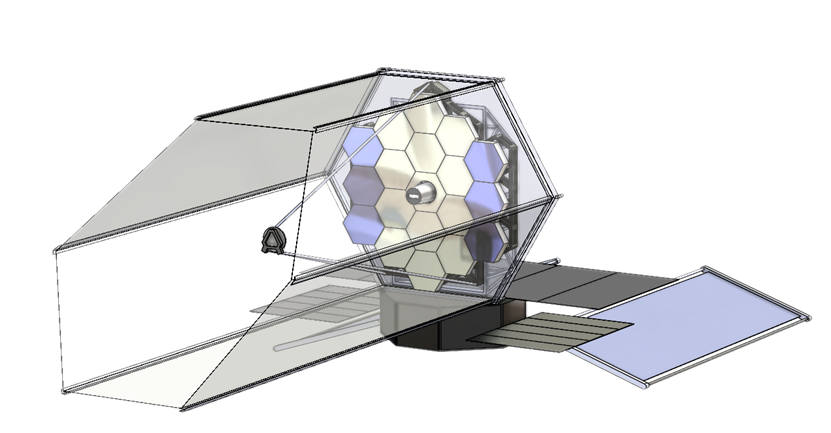
\includegraphics[width=\textwidth]{3.5ST_in_KASI.png}
  \vspace*{\stretch{2.2}}
  \noindent\colorbox{Blue3}{\parbox[t]{\dimexpr\textwidth-2\fboxsep\relax}{%
    \vspace{3mm}\centering
    {\color{white}\bfseries\Large 3.5-meter Segmented-Mirror Robotic Space Telescope}\\[1.5mm]
    {\color{white!88}\normalsize Korea Astronomy and Space Science Institute}%
    \vspace{3mm}}}
  \vspace{3mm}
  \clearpage}
